% TODO: add support for Lumos-compatible RS-485 protocol
\input common
\frontmatter
\definecolor{reservedslot}{gray}{0.8}
\newcommand\api{\acronym{API}}
\newcommand\pc{\acronym{PC}}
\newcommand\cli{\acronym{CLI}}
\newcommand\ascii{\acronym{ASCII}}
\newcommand\led{\acronym{LED}}
\newcommand\codetype[1]{\z{#1}}
\newcommand\ixz[1]{\index{#1@\z{#1}}\z{#1}}
\newcommand\tUnused{\cellcolor{gray!50}}
\newcommand\tControl{\cellcolor{yellow!50}}
\newcommand\tForbidden{\cellcolor{red!50}}
\newcommand\tSpecial{\cellcolor{blue!25}}
%\colorlet{tableheader}{blue!40}
%\colorlet{tablesubhead}{blue!20}
%\colorlet{recordbox}{blue!15}
%\colorlet{recordtext}{black}
%\usetikzlibrary{positioning,shapes,shadows,arrows}
%\tikzstyle{program}=[rectangle, draw=black, rounded corners, fill=recordbox, drop shadow,
%	anchor=north, text=recordtext, text width=2cm]
%\tikzstyle{instance}=[rectangle, draw=black, rounded corners, fill=green!15, drop shadow,
%	anchor=north, text=black, text width=3cm]
%\tikzstyle{line}=[-, thick]
%\tikzstyle{myarrow}=[->, >=triangle 45, thick]
\hypersetup{
	pdftitle={Readerboard User's Guide},
	pdfkeywords={Open Source Readerboard Hardware and Software},
	pdfauthor={Steve Willoughby / Mad Science Zone},
	pdfsubject={Readerboard Project Documentation * (c) 2023 * Creative Commons Licensing (See Document for details)},
	colorlinks=true,
	linkcolor=blue!30!black,
}
\thispagestyle{empty}
	\begin{center}
		\Huge Readerboard \\ User's Guide \\
		WORKING\\DRAFT
	\end{center}

\vfill
%\end{flushright}
\newpage
The information in this document, and the hardware and software it describes, are hobbyist
works created as an educational exercise and as a matter of personal interest for recreational
purposes.

It is not to be considered an industrial-grade or retail-worthy product.
It is assumed that the user has the necessary understanding and skill to use it appropriately.  The author makes NO
representation as to suitability or fitness for any purpose whatsoever, and disclaims any and all liability or 
warranty to the full extent permitted by applicable law.  It is explicitly not designed for use where the safety
of persons, animals, property, or anything of real value depends on the correct operation of the software.

\strut\vfill

\begin{center}\bfseries
	For readerboard hardware version 2.1.0, and firmware version 0.0.0.
\end{center}

\strut\vfill

\noindent Copyright \copyright\ 2023 by Steven L. Willoughby
(aka MadScienceZone), Aloha, Oregon, USA. All Rights Reserved.
This document is released under the terms and conditions of the
Creative Commons ``Attribution-NoDerivs 3.0 Unported'' license.
In summary, you are free to use, reproduce, and redistribute this 
document provided you give full attribution to its author and do not
alter it or create derivative works from it.  See
\begin{center}
\href{http://creativecommons.org/licenses/by-nd-3.0}{http://creativecommons.org/licenses/by\-nd\-/\-3.0/} 
\end{center}
for the full set of licensing terms.

\begin{center}
\LJimg[width=.25in]{cc}\LJimg[width=.25in]{by}\LJimg[width=.25in]{nd}
\end{center}

\newpage
\tableofcontents
\newpage
\listoffigures
\listoftables
\mainmatter

%%%%%%%%%%%%%%%%%%%%%%%%%%%%%%%%%%%%%%%%%%%%%%%%%%%%%%%%%%%%%%%%%%%%%%%%%%%%%%%%%%%%%%%%%%%%%%%%%%%%
%  _   _    _    ____  ______        ___    ____  _____ 
% | | | |  / \  |  _ \|  _ \ \      / / \  |  _ \| ____|
% | |_| | / _ \ | |_) | | | \ \ /\ / / _ \ | |_) |  _|  
% |  _  |/ ___ \|  _ <| |_| |\ V  V / ___ \|  _ <| |___ 
% |_| |_/_/   \_\_| \_\____/  \_/\_/_/   \_\_| \_\_____|
%
\chapter{Hardware}
\epigraph{People who are really serious about software should make their own hardware.}{---Alan Kay}
\LJversal{A}{s a hobby project,} the design of the hardware and software for the readerboard
project ``grew in the telling'' as new ideas sprang to mind. As of this writing, there are three
different models of hardware prototypes which were designed and created.

\section{Version 1.0.1}
The initial prototype was a fairly large board, approximately 20\sfrac{5}{8}$\times$6\sfrac{5}{8}$''$
with an \acronym{LED} pitch of \sfrac{1}{3}$''$.

It requires an Arduino Mega 2560 or Arduino Due to drive it. A custom-made shield board attaches to
the Arduino, which provides connectors for power and ribbon cables to drive the display (one to control
the matrix, the other for the 8 status \acronym{LED}s which appear in a horizontal row along the bottom
right of the matrix).

%One of the problems with this board is the use of the obsolete \acronym{TPIC6B595} chip. Later boards
%replaced this with a newer version. While it's technically possible to use the newer \acronym{STPIC6D595} chips
%on the 1.0.1 board, doing so requires a non-standard placement of the newer chip on the older chip's pads, 
%bending pins up, soldering jumper wires, possibly cutting traces, and and due
%to a pinout incompatibility between the two chips, the firmware also needs to be altered. As such, we don't
%recommend going this route. It would be best to use the newer board with the chips it was designed for.

\section{Version 2.0.0}
This version is based on the 1.0.1 design, but shrunk to a board size of about 18\sfrac{3}{16}$\times$5\sfrac{3}{16}$''$
with an \acronym{LED} pitch of \sfrac{1}{4}$''$. It also replaces the obsolete \acronym{TPIC6B595} with the newer \acronym{STPIC6D595} chip.
It also relocates the ribbon cable which connects the Arduino controller to the \acronym{LED} matrix, moves the
eight status \acronym{LED}s to a vertical column to the right of the matrix, and switches to resistor arrays
for the matrix current limiting resistors, instead of the individual discrete resistors used on the 1.0.1 board.

\section{Version 2.1.0}
Version 2.1.0 is a significant change to the 2.0.0 board in terms of how it interfaces with the Arduino, although it has the same size and physical
layout as the 2.0.0 board.

This one eliminates the need for the ribbon cables and shield board. Instead, the Arduino controller mounts
directly to the back of the display board. This means that the lower portion of the left edge of the enclosure
has all of the external connections in one place, including power, \acronym{RS-485} in and out, and the 
\acronym{USB} connector(s) on the Arduino itself.

\section{Firmware Implications}
The boards for versions 1.0.1 and 2.0.0 were compatible and used the same Arduino shield. Thus, they
use the same firmware images. The 2.1.0 board, however, which integrates the Arduino directly instead
of using a separate shield with ribbon cables, assigns signals to different I/O pins, and as such
needs a different firmware image. 

Both images are generated from the same source files, with compile-time switches to make one or the other.

                                                      
%%%%%%%%%%%%%%%%%%%%%%%%%%%%%%%%%%%%%%%%%%%%%%%%%%%%%%%%%%%%%%%%%%%%%%%%%%%%%%%%%%%%%%%%%%%%%%%%%%%%
%  ____  ____   ___ _____ ___   ____ ___  _     
% |  _ \|  _ \ / _ \_   _/ _ \ / ___/ _ \| |    
% | |_) | |_) | | | || || | | | |  | | | | |    
% |  __/|  _ <| |_| || || |_| | |__| |_| | |___ 
% |_|   |_| \_\\___/ |_| \___/ \____\___/|_____|
%
\chapter{Protocol Description}\label{chap:protocol}
{\setlength{\epigraphwidth}{.5\textwidth}
\epigraph{I don't stand on protocol. Just call me your Excellency.}{---Henry Kissinger}}
\LJversal{T}{he control protocol} used to display information on the readerboard sign is very simple.
Commands are expressed largely in plain \ascii\ characters and are executed immediately
as they are received.\footnote{Technically, they may even be executed \emph{while} they
are being received.}
%It is not necessarily required for a command to be fully received first,
%so it is possible that the sign will have started operating on part of the command (e.g.,
%moving the current cursor column position) even if the rest of the command could not be
%performed.

In addition to plain, printable 7-bit \ascii\ characters, a few control codes are
recognized as described below. String data may include any 8-bit value except as otherwise
indicated.

\section{USB vs. RS-485}
The protocol used to send commands to the readerboard is different depending on
whether the host is sending directly to a single readerboard over a \acronym{USB}
cable, or to (possibly) multiple readerboards over an RS-485 bus network.

\subsection{USB}
A readerboard connected via \acronym{USB} accepts the commands just as documented
below, with the addition that each such command is terminated by a 
\z{\textasciicircum D} byte (hex value \z{04}$_{16}$).
\begin{center}
\begin{bytefield}[endianness=little,bitwidth=0.11111\textwidth]{9}
	\bitbox[]{1}{\scriptsize0}&
	\bitbox[]{1}{\scriptsize\dots}&
	\bitbox[]{1}{\scriptsize$n-1$}&
	\bitbox[]{1}{\scriptsize$n$}\\
	\bitbox{3}{\Var*{command}}&
	\bitbox{1}{\z{\textasciicircum D}}
\end{bytefield}
\end{center}

If there is an error parsing or executing a command, the readerboard will ignore
all subsequent input until a \z{\textasciicircum D} is received, whereupon it will
expect to see the start of another command. Thus, \z{\textasciicircum D} may not
appear in any transmitted data except to terminate commands.

\subsection{RS-485}
Commands sent over RS-485 are intended to target one or more of a set of
connected readerboards over a network which may also contain other Lumos-protocol-compatible
devices, so they adhere to a protocol that is also compatible with those devices.

Each command begins with one of the following binary headers, depending on the
set of target readerboard signs which should obey the command.

\subsubsection{Single Target or All Readerboards}
To send a command to a single sign, begin with a single byte encoded as:
\begin{center}
	\begin{bytefield}[endianness=big]{8}
		\bitheader{0-7} \\
		\bitbox{1}{\z{1}}&
		\bitbox[tbl]{1}{\z0}&
		\bitbox[tb]{1}{\z0}&
		\bitbox[tbr]{1}{\z1}&
		\bitbox{4}{\Var*{ad}}
	\end{bytefield}
\end{center}
where \Var*{ad} is the sign's address on the bus, which must be a value in the
range 0--15. This byte is followed by any command as described below. 
If the global address \Var{ad$_G$} is given as the \Var*{ad} value, then all readerboards
which have that set as their global address will obey the command.

\subsubsection{Multiple Targets}
Alternatively, a command may be targeted to multiple signs by starting the command
with a multi-byte code:
\begin{center}
	\begin{bytefield}[endianness=big]{8}
		\bitheader{0-7} \\
		\bitbox{1}{\z{1}}&
		\bitbox[tbl]{1}{\z0}&
		\bitbox[tb]{1}{\z1}&
		\bitbox[tbr]{1}{\z1}&
		\bitbox{4}{\Var*{ad$_G$}}\\
		\bitbox{1}{\z0}&
		\bitbox{1}{\z0}&
		\bitbox{6}{\Var*{n}}\\
		\bitbox{1}{\z0}&
		\bitbox{1}{\z0}&
		\bitbox{6}{\Var*{ad$_0$}}\\
		\bitbox[]{8}{$\vdots$\strut}\\
		\bitbox{1}{\z0}&
		\bitbox{1}{\z0}&
		\bitbox{6}{\Var*{ad$_{n-1}$}}
	\end{bytefield}
\end{center}
where \Var*{ad$_G$} is the ``global'' device address which signals readerboards
generally (see the \z= command below).
This will send to the \Var*{n} devices addressed as \Var*{ad$_0$} through \Var*{ad$_{n-1}$}.

Note that device addresses are constrained to the range 0--15 if they are to be addressed in
the command start byte. However, using the multiple target header, device addresses in the
range 0--63 may be used.

%\subsubsection{All Targets}
%If you wish to send a command to all attached readerboards, simply send the
%following byte ahead of the command:
%\begin{center}
%	\begin{bytefield}[endianness=big]{8}
%		\bitheader{0-7} \\
%		\bitbox{1}{\z{1}}&
%		\bitbox[tbl]{1}{\z1}&
%		\bitbox[tb]{1}{\z0}&
%		\bitbox[tbr]{1}{\z1}&
%		\bitbox{4}{\Var*{ad$_G$}}
%	\end{bytefield}
%\end{center}
%where \Var*{ad$_G$} is the ``global'' device address which signals readerboards
%generally (see the \z= command below).

\subsubsection{All Off}
As a special case, the single byte
\begin{center}
	\begin{bytefield}[endianness=big]{8}
		\bitheader{0-7} \\
		\bitbox{1}{\z{1}}&
		\bitbox[tbl]{1}{\z0}&
		\bitbox[tb]{1}{\z0}&
		\bitbox[tbr]{1}{\z0}&
		\bitbox{4}{\Var*{ad}}
	\end{bytefield}
\end{center}
will cause the readerboard addressed as \Var*{ad} to turn off all \led s.
If \Var*{ad} is the \Var{ad$_G$} address, then all readerboards will turn off
all \led s.

No other command bytes need to follow; this byte is sufficient to turn off
the sign(s).

\subsubsection{Subsequent Command Bytes}
All subsequent bytes which follow the above binary headers \emph{must} have their
\acronym{MSB} cleared to \z0. 

To cover cases where a value sent as part of a command must have the \acronym{MSB}
set, we use the following escape codes:
\begin{itemize}
	\item A hex byte \z{7E}$_{16}$ causes the next byte received to have its
		\acronym{MSB} set upon receipt.
	\item A hex byte \z{7F}$_{16}$ causes the next byte to be accepted without
		any further interpretation.
\end{itemize}
Thus, the byte \z{C4}$_{16}$ is sent as the two-byte sequence \z{7E~44},
while a literal \z{7E} is sent as \z{7F~7E} and a literal \z{7F} as \z{7F~7F}.

If there is an error parsing or executing a command, the readerboard will ignore
all subsequent input until a byte arrives with its \acronym{MSB} set to \z1,
whereupon it will expect to see the start of another command. 

A few illustrative examples are shown in Table~\ref{tbl:escapes}.
\begin{table}
	\begin{center}
		\begin{tabular}{ll}\toprule
			\multicolumn{1}{c}{\bfseries Input Sequence}&
			\multicolumn{1}{c}{\bfseries Resulting Byte}\\\midrule
			\z{00}    & \z{00} \\
			\z{7D}    & \z{7D} \\
			\z{7F 7E} & \z{7E} \\
			\z{7F 7F} & \z{7F} \\
			\z{7E 00} & \z{80} \\
			\z{7E 01} & \z{81} \\
			\z{7E 7D} & \z{FD} \\
			\z{7E 7E} & \z{FE} \\
			\z{7E 7F} & \z{FF} \\\bottomrule
		\end{tabular}
		\caption{Examples of RS-485 Escape Bytes.\label{tbl:escapes}}
	\end{center}
\end{table}

%\section{Command Addressing}
%Commands may be received over the \acronym{USB} port (a point-to-point connection with a host computer)
%or the RS-485 port (as part of a network of devices all connected to a single host computer's port).
%Commands received over the \acronym{USB} port \mc{MAY} be prefixed by an address specifier as described
%below. Those received over the RS-485 network \mc{MUST} have such a prefix (unless 
%using Lumos-compatible mode as described below).
%
%The address specifier prefix has the form:
%\begin{center}
%\begin{bytefield}[endianness=little,bitwidth=0.11111\textwidth]{9}
%	\bitbox[]{1}{\scriptsize0}&
%	\bitbox[]{1}{\scriptsize1}&
%	\bitbox[]{1}{\scriptsize\dots}&
%	\bitbox[]{1}{\scriptsize$n$}&
%	\bitbox[]{1}{\scriptsize$n+1$}\\
%	\bitbox{1}{\z{/}} &
%	\bitbox[tbl]{1}{\Var*{ad$_0$}}&
%	\bitbox[tb]{1}{$\cdots$}&
%	\bitbox[tbr]{1}{\Var*{ad$_{n-1}$}}&
%	\bitbox{1}{\z{\$}}
%\end{bytefield}
%\end{center}
%
%The \Var*{ad} parameters give the address(es) of the sign(s) which should obey the following
%command. Each is a value from 0--63 encoded as shown in Table~\ref{tbl:int063}. If the list of
%addresses is empty,
%all signs should respond to the command. The address list
%terminator may be a dollar-sign or escape
%character (hex byte \z{1B}), indicated in the protocol description as \z{\$}.
%
%If sent over the \acronym{USB} port, the address prefix is allowed but ignored, and the readerboard
%acts as if all commands are addressed to it, since the commands are received over a private connection
%between the host and that readerboard.
%
%If sent over the RS-485 port, the following escape codes are recognized.
%To send a byte value greater than 127, it is necessary to send it as the two-byte sequence:
%\begin{center}
%	\begin{bytefield}[endianness=big]{8}
%		\bitheader{0-7} \\
%		\bitbox{1}{\z0}&
%		\bitbox[tbl]{1}{\z1}&
%		\bitbox[tb]{1}{\z1}&
%		\bitbox[tb]{1}{\z1}&
%		\bitbox[tb]{1}{\z1}&
%		\bitbox[tb]{1}{\z1}&
%		\bitbox[tb]{1}{\z1}&
%		\bitbox[tbr]{1}{\z0}\\
%		\bitbox{1}{\z0}&
%		\bitbox{7}{\Var*{x}}
%	\end{bytefield}
%\end{center}
%This accepts the byte \Var*{x}, with its \acronym{MSB} set to \z1.
%
%To send a literal value of \z{7E}$_{16}$ rather than having it start the above
%escape, simply start with the other escape sequence:
%\begin{center}
%	\begin{bytefield}[endianness=big]{8}
%		\bitheader{0-7} \\
%		\bitbox{1}{\z0}&
%		\bitbox[tbl]{1}{\z1}&
%		\bitbox[tb]{1}{\z1}&
%		\bitbox[tb]{1}{\z1}&
%		\bitbox[tb]{1}{\z1}&
%		\bitbox[tb]{1}{\z1}&
%		\bitbox[tb]{1}{\z1}&
%		\bitbox[tbr]{1}{\z1}\\
%		\bitbox{1}{\z0}&
%		\bitbox{7}{\Var*{y}}
%	\end{bytefield}
%\end{center}
%This accepts the byte \Var*{y}, without interpreting it further. Thus, to send
%the hex byte \z{7E}, you send the two bytes \z{7F~7E}. To send a literal \z{7F}
%byte, send the two bytes \z{7F~7F}.
%
%The readerboard \acronym*{MAY} accept 8-bit values in the range 128--255 (hex
%\z{80}--\z{FF}) without using these escape codes, but this will confuse any other
%Lumos-compatible devices on the same serial network with them, so the best practice
%is to always use these escape codes for any value greater than or equal to 126 (hex
%\z{7E}). If using with other Lumos devices, you \acronym*{MUST} do so.
%
%\section{Lumos Compatibility}
%The readerboard may be connected to an RS-485 network that includes Lumos-protocol
%devices.\footnote{These include the Lumos power control boards and quiz show equipment
%created by the author.} 
%
%In this case, readerboard commands must begin with a start byte in the form
%\begin{center}
%	\begin{bytefield}[endianness=big]{8}
%		\bitheader{0-7} \\
%		\bitbox{1}{\z{1}}&
%		\bitbox{3}{\Var*{cmd}}&
%		\bitbox{4}{\Var*{ad$_0$}}
%	\end{bytefield}
%\end{center}
%and the address \Var*{ad$_0$} must be in the range 0--15. In this mode, all following
%bytes sent to the readerboard must have their \acronym{MSB} cleared (\z0).
%
%Only two \Var*{cmd} values are recognized by the readerboard.  For compatibility with
%other Lumos devices which recognize \Var*{cmd}=0 to mean turn off all output, the single-byte command
%\begin{center}
%	\begin{bytefield}[endianness=big]{8}
%		\bitheader{0-7} \\
%		\bitbox{1}{\z1}&
%		\bitbox[tbl]{1}{\z0}&
%		\bitbox[tb]{1}{\z0}&
%		\bitbox[tbr]{1}{\z0}&
%		\bitbox{4}{\Var*{ad$_0$}}
%	\end{bytefield}
%\end{center}
%will cause the readerboard addressed as \Var*{ad$_0$} to immediately turn off all
%\led s.
%
%For any other readerboard command, the start byte must be
%\begin{center}
%	\begin{bytefield}[endianness=big]{8}
%		\bitheader{0-7} \\
%		\bitbox{1}{\z{1}}&
%		\bitbox[tbl]{1}{\z1}&
%		\bitbox[tb]{1}{\z0}&
%		\bitbox[tbr]{1}{\z1}&
%		\bitbox{4}{\Var*{ad$_0$}}
%	\end{bytefield}
%\end{center}
%
%This may be followed by an address specifier (starting with a ``\z/'' character)
%documented above to include more sign addresses other than \Var*{ad$_0$}. If no such
%specifier is sent, then only sign \Var*{ad$_0$} will act on the command. If an empty
%specifier is sent, then \emph{all} signs will act on it.
%
%That is
%then followed by any of the readerboard commands documented below.\footnote{This
%is cheating just a little bit but is based on the assumption that no other Lumos
%device on any address will have \Var*{cmd} value 5 with the next byte being a
%``\z/'' character followed by zero or more encoded values 0--63 and an escape or
%dollar-sign.}
%
%\section{Command Termination and Error Handling}
%The command terminator is ``\z{\textasciicircum D}'' (hex byte value \z{04}). %We
%%\emph{recommend} that every command---or group of commands which together represent
%%a logical update to the sign---be followed by a \z{\textasciicircum D} character.
%This character \emph{must} follow each readerboard command, since the interpretation
%of the next command won't start until receipt of the 
%\z{\textasciicircum D},
%effectively
%ignoring any data sent after the end of the command and before the terminating
%\z{\textasciicircum D}.
%
%The exception to this rule is the set of Busylight-compatible commands
%\z*,
%\z?,
%\z{F},
%\z{S},
%and
%\z{X}.
%Since the Busylight unit did not use any command terminator in its protocol, the readerboard
%unit won't demand one either, although we \emph{recommend} that you do anyway. At the very least,
%you should have a
%\z{\textasciicircum D}
%character sent after a sequence of one or more Busylight-compatible commands.
%
%%The individual commands are executed immediately upon receipt, without requiring the
%%\z{\textasciicircum D} byte. For example, in the sequence ``\z{H1H2H3\textasciicircum D}''
%%the first bar graph data point will be displayed as soon as ``\z{H1}'' is received.
%
%In case of an error, such as the inability to parse the incoming command or an invalid
%field value, the readerboard will signal the error condition by lighting the white and
%both red discrete \led s, and will then ignore all input until the next
%\z{\textasciicircum D} byte is received.
%
%Whenever a \z{\textasciicircum D} byte is received, any command being parsed is aborted
%and the sign's input parser is reset. Thus, this byte may be sent in case a partial command
%has been sent but the host becomes aware that it cannot be completed. Note that the command
%may have been partially acted upon by that point, so no assumption should be made as to the
%sign's state.
%
%In the descriptions that follow, a trailing \z{\textasciicircum D} is shown at the end
%of each command to remind you of the recommendation to send this terminator, even though
%the commands themselves do not require them, strictly speaking.

\section{Command Summary}
The eight discrete \led s are intended for a simple display of status information
in a manner analogous to the Busylight project by the same author.\footnote{See
\href{https://github.com/MadScienceZone/busylight}{github.com/MadScienceZone/busylight}.}
To support this usage, the \z{F}, \z{S}, \z{X}, \z*, and \z? commands are recognized
in a manner compatible with how Busylight uses those same commands. These are categorized
as ``Busylight compatibility commands.'' Unlike all other commands listed here, these are
recognized regardless of case.  Since the readerboard has a power supply capable of illuminating
all of the status \led s at once,\footnote{The Busylight cannot, since it is powered
from the host computer's \acronym{USB} port.} a new command \z{L} is added which allows any
arbitrary pattern of steady \led s to be turned on.

The remaining commands are used for management of the matrix display. All commands are summarized in Table~\ref{tbl:commands}.
\begin{table}
	\begin{center}
		\begin{tabular}{cll}\toprule
			\multicolumn{1}{c}{\bfseries Command}&
			\multicolumn{1}{c}{\bfseries Description}&
			\multicolumn{1}{c}{\bfseries Notes}\\\midrule
			\z{*} & Strobe \led s in Sequence & [1]\\
			\z{?} & Query discrete \led\ status & [1] [2] [4]\\
			\z{F} & Flash \led s in Sequence & [1]\\
			\z{L} & Light one or more \led s steady & [3]\\
			\z{S} & Light one \led\ steady & [1]\\
			\z{X} & All \led s off & [1]\\
			\midrule
			\z{\textasciicircum D} & Abort/terminate command & \\
			\z{<} & Scroll text across display & \\
			\z{=} & Set operational parameters & [4]\\
			\z{@} & Move current column cursor & \\
			\z{A} & Select character font & \\
			\z{C} & Clear matrix display & \\
			\z{H} & Add histogram/bargraph data point & \\
			\z{I} & Draw bitmap graphic image & \\
			\z{K} & Set current color & \\
			\z{Q} & Query matrix display status & [2] [4]\\
			\z{T} & Display text on display & \\
			\bottomrule
			\multicolumn{3}{l}{\footnotesize [1] Busylight compatibile command}\\
			\multicolumn{3}{l}{\footnotesize [2] Sends response (\acronym{USB} only)}\\
			\multicolumn{3}{l}{\footnotesize [3] Busylight extension (not in original Busylight)}\\
			\multicolumn{3}{l}{\footnotesize [4] \acronym{USB} only}\\
		\end{tabular}
		\caption{Summary of All Commands\label{tbl:commands}}
	\end{center}
\end{table}

Although the rev 2 hardware supports the ability to enable the RS-485 transmitter and send data back onto the network,
this is not currently implemented by the firmware, and the intent is to have all devices listen passively to RS-485 traffic
at all times.

\section{\z{*}---Strobe Lights in Sequence}
\begin{center}
\begin{bytefield}[endianness=little,bitwidth=0.11111\textwidth]{7}
%	\bitheader{0-3} \\
	\bitbox[]{1}{\scriptsize0}&
	\bitbox[]{1}{\scriptsize1}&
	\bitbox[]{1}{\scriptsize2}&
	\bitbox[]{1}{\scriptsize3}&
	\bitbox[]{1}{\scriptsize\dots}&
	\bitbox[]{1}{\scriptsize$n$}&
	\bitbox[]{1}{\scriptsize$n+1$}\\
	\bitbox{1}{\z{*}} &
	\bitbox[tlb]{1}{\Var*{led$_0$}} &
	\bitbox[tb]{1}{\Var*{led$_1$}} &
	\bitbox[tb]{1}{\Var*{led$_2$}} &
	\bitbox[tb]{1}{$\cdots$} &
	\bitbox[tbr]{1}{\Var*{led$_{n-1}$}} &
	\bitbox{1}{\z\$}
\end{bytefield}
\end{center}

Each \Var*{led} value is an \ascii\ character corresponding to a discrete
\led\ as shown in Table~\ref{tbl:lightcodes}. An \Var*{led} value of ``\z{\_}'' means
there is no \led\ illuminated at that point in the sequence.

This command functions identically to the \z{F} command (see below), except that the lights
are ``strobed'' (flashed very briefly with a pause between each light in the sequence).

\section{\z<---Scroll Text Across Display}
\begin{center}
\begin{bytefield}[endianness=little,bitwidth=0.11111\textwidth]{8}
%	\bitheader{0-8} \\
	\bitbox[]{1}{\scriptsize0}&
	\bitbox[]{1}{\scriptsize1}&
	\bitbox[]{1}{\scriptsize2}&
	\bitbox[]{3}{\scriptsize\dots}&
	\bitbox[]{1}{\scriptsize$n$+1}&
	\bitbox[]{1}{\scriptsize$n$+2}\\
	\bitbox{1}{\z{<}} &
	\bitbox{1}{\Var*{loop}}&
	\bitbox{5}{\Var*{string}}&
	\bitbox{1}{\z{ESC}}
\end{bytefield}
\end{center}

Displays the text \Var*{string} by scrolling it across the display from right to left.
If \Var*{loop} is ``\z.'', the text is only scrolled once; if it is ``\z{L}'' then it
repeatedly scrolls across the screen in an endless loop.

The text is rendered in the current font and may contain any 8-bit bytes except as otherwise
noted (but avoiding \ascii\ control codes is wise to be safe from conflict with
future control codes which may be added to the protocol). The string is terminated by an
escape character (hex byte \z{1B}), indicated in the protocol description as \z{ESC}.

The string may include control codes as listed in Table~\ref{tbl:controlcodes}.
\begin{table}
	\begin{center}
		\begin{tabular}{lll}\toprule
			\multicolumn{1}{c}{\bfseries Code} &
			\multicolumn{1}{c}{\bfseries Hex} &
			\multicolumn{1}{c}{\bfseries Description} \\\midrule
			\z{\textasciicircum C}\Var*{pos} & \z{03}\Var*{pos} & Move current column cursor to \Var*{pos}\\
			\z{\textasciicircum D} & \z{04} & Never allowed in strings (command terminator)\\
			\z{\textasciicircum F}\Var*{digit} & \z{06}\Var*{digit} & Switch current font\\
			\z{\textasciicircum H}\Var*{pos} & \z{08}\Var*{pos} & Move cursor left \Var*{pos} columns\\
			\z{\textasciicircum K}\Var*{rgb} & \z{0B}\Var*{rgb} & Change color to \Var*{rgb}\\
			\z{\textasciicircum L}\Var*{pos} & \z{0C}\Var*{pos} & Move cursor right \Var*{pos} columns\\
			\z{\textasciicircum [} & \z{1B} & Never allowed in strings (string terminator)\\
			\bottomrule
		\end{tabular}
		\caption{Control Codes in String Values\label{tbl:controlcodes}}
	\end{center}
\end{table}

\section{\z{=}---Set Operational Parameters}
\begin{center}
\begin{bytefield}[endianness=little,bitwidth=0.11111\textwidth]{8}
%	\bitheader{0-3} \\
	\bitbox[]{1}{\scriptsize0}&
	\bitbox[]{1}{\scriptsize1}&
	\bitbox[]{1}{\scriptsize2}&
	\bitbox[]{1}{\scriptsize3}&
	\bitbox[]{1}{\scriptsize4}\\
	\bitbox{1}{\z{=}} &
	\bitbox{1}{\Var*{ad}}&
	\bitbox{1}{\Var*{uspd}}&
	\bitbox{1}{\Var*{rspd}}&
	\bitbox{1}{\Var*{ad$_G$}}
\end{bytefield}
\end{center}

This command sets a few operational parameters for the sign. Once set, these will be persistent across
power cycles and reboots.

If the \Var*{ad} parameter is ``\z{\_}'' then the RS-485 interface is disabled entirely. Otherwise it is a
value from 0--15 encoded as described in Table~\ref{tbl:int063}. This enables the RS-485 interface and assigns
this sign's address to \Var*{ad}.

The baud rate for the \acronym{USB} and RS-485 interfaces is set by the \Var*{uspd} and \Var*{rspd} values
respectively. Each is encoded as per Table~\ref{tbl:baudcodes}.

The \Var*{ad$_G$} value is an address in the range 0--15 which is not assigned
to any other device on the RS-485 network. This is used to signal that all
readerboards should pay attention to the start of the command because it might
target them either as part of a list of specific readerboards or because the
command is intended for all readerboards at once. This is encoded in the 
same way as \Var*{ad}.
If you only have one readerboard or do no wish to assign a global address,
just set \Var*{ad$_G$} to the same value as \Var*{ad}.

This command may only be sent over the \acronym{USB} port.

By default, an unconfigured readerboard is set to 9,600 baud with the RS-485 port disabled.
\begin{table}
	\begin{center}
		\begin{tabular}{crl}\toprule
			\bfseries Code & \multicolumn{1}{c}{\bfseries Speed} \\\midrule
			0 & 300\\
			1 & 600\\
			2 & 1,200\\
			3 & 2,400\\
			4 & 4,800\\
			5 & 9,600 & (default)\\
			6 & 14,400\\
			7 & 19,200\\
			8 & 28,800\\
			9 & 31,250\\
			A & 38,400\\
			B & 57,600\\
			C & 115,200\\
		\bottomrule
		\end{tabular}
		\caption{Baud Rate Codes\label{tbl:baudcodes}}
	\end{center}
\end{table}

\section{\z?---Query Discrete \led\ Status}
\begin{center}
\begin{bytefield}[endianness=little,bitwidth=0.11111\textwidth]{1}
	\bitheader{0} \\
	\bitbox{1}{\z{?}}
\end{bytefield}
\end{center}

This command causes the sign to send a status report back to the host to indicate
what the discrete \led s are currently showing. This response has the form:

\medskip

\begin{center}\begin{bytefield}[endianness=little,bitwidth=0.11111\textwidth]{9}
	\bitheader{0-8} \\
	\bitbox{1}{\z{L}} &
	\bitbox[tbl]{1}{\Var*{led$_0$}} &
	\bitbox[tb]{1}{\Var*{led$_1$}} &
	\bitbox[tb]{1}{\Var*{led$_2$}} &
	\bitbox[tb]{1}{\Var*{led$_3$}} &
	\bitbox[tb]{1}{\Var*{led$_4$}} &
	\bitbox[tb]{1}{\Var*{led$_5$}} &
	\bitbox[tb]{1}{\strut$\cdots$} &
	\bitbox[tbr]{1}{\Var*{led$_{n-1}$}} \\
	\bitbox{1}{\z{\$}} &
	\bitbox{1}{\z{F}} &
	\bitbox{7}{flasher status (see below)} \\
	\bitbox{1}{\z{\$}} &
	\bitbox{1}{\z{S}} &
	\bitbox{7}{strober status (see below)} \\
	\bitbox{1}{\z{\$}} &
	\bitbox{1}{\z{\textbackslash n}}
\end{bytefield}
\end{center}

Each \Var*{led$_x$} value is a single character which is ``\z{\_}'' if the corresponding \led\ is
off, or the \led's color code or position number if it is on. One such value is sent for each \led\ installed
in the sign (typically eight for readerboards), followed by a ``\z{\$}'' to mark the end of the list.

The flasher and strober status values are variable-width fields which indicate the
state of the flasher (see \z{F} command) and strober (see \z{*} command) functions.
In each case, if there is no defined sequence, the status field will be:

\medskip

\begin{center}\begin{bytefield}[endianness=little,bitwidth=0.11111\textwidth]{2}
	\bitheader{0-1} \\
	\bitbox{1}{\Var*{run}} &
	\bitbox{1}{\strut\z{\_}}
\end{bytefield}
\end{center}

\smallskip

\noindent Otherwise, the state of the flasher or strober unit is indicated by:

\medskip

\begin{center}\begin{bytefield}[endianness=little,bitwidth=0.11111\textwidth]{7}
%	\bitheader{0-6} \\
	\bitbox[]{1}{\scriptsize0}&
	\bitbox[]{1}{\scriptsize1}&
	\bitbox[]{1}{\scriptsize2}&
	\bitbox[]{1}{\scriptsize3}&
	\bitbox[]{1}{\scriptsize4}&
	\bitbox[]{1}{\scriptsize\dots}&
	\bitbox[]{1}{\scriptsize$n+3$}\\
	\bitbox{1}{\Var*{run}} &
	\bitbox{1}{\Var*{pos}} &
	\bitbox{1}{\z{@}} &
	\bitbox[tbl]{1}{\Var*{led$_0$}} &
	\bitbox[tb]{1}{\Var*{led$_1$}} &
	\bitbox[tb]{1}{$\cdots$} &
	\bitbox[tbr]{1}{\Var*{led$_{n-1}$}} 
\end{bytefield}
\end{center}

In either case, \Var*{run} is the \ascii\ character ``\z{S}'' if the unit is
stopped or ``\z{R}'' if it is currently running.  If there is a defined sequence,
\Var*{pos} indicates the 0-origin position within the sequence of the light currently
being flashed or strobed, encoded as described in Table~\ref{tbl:int063}. 
The \Var*{led$_x$} values are as allowed for the \z{F} or \z{*}
command that set the sequence. (Regardless of the actual \z{F} or \z{*} command parameters,
the report will show symbolic color codes where possible, or numeric position codes otherwise.)

%Note that the \Var*{pos} value may be the character ``\z{X}'' to indicate the position
%value of 40, so it is important to distinguish between the field value
%``\Var*{run}\z{X}'' vs.\@ ``\Var*{run}\z{X@}\Var*{sequence}''.

The status message sent to the host is terminated by a newline character (hex byte \z{0A}),
indicated in the protocol description above as ``\z{\textbackslash n}''.
\begin{table}
	\begin{center}
		\begin{tabular}{cc|cc}\toprule
			\multicolumn{1}{c}{\bfseries Value} &
			\multicolumn{1}{c}{\bfseries Code} &
			\multicolumn{1}{c}{\bfseries Value} &
			\multicolumn{1}{c}{\bfseries Code} \\\midrule
			0--9 & \z0--\z9 & 17--42 & \z{A}--\z{Z} \\
			10 & \z: & 43 & \z[ \\
			11 & \z; & 44 & \z\textbackslash \\
			12 & \z< & 45 & \z] \\
			13 & \z= & 46 & \z\textasciicircum \\
			14 & \z> & 47 & \z{\_} \\
			15 & \z? & 48 & \z` \\
			16 & \z@ & 49--63 & \z{a}--\z{o} \\
			\bottomrule
		\end{tabular}

		{\footnotesize (Each code is the numeric value plus 48.)}
		\caption{\ascii\ Encoded Integer Values (0--63)\label{tbl:int063}}
	\end{center}
\end{table}

This command may only be sent on the \acronym{USB} port.

\section{\z{@}---Set Column Cursor Position}
\begin{center}
\begin{bytefield}[endianness=little,bitwidth=0.11111\textwidth]{2}
	\bitheader{0-1} \\
	\bitbox{1}{\z{@}} &
	\bitbox{1}{\Var*{pos}} 
\end{bytefield}
\end{center}

Sets the column cursor position to the value indicated by \Var*{pos}. See Table~\ref{tbl:int063}.

\section{\z{A}---Select Font}
\begin{center}
\begin{bytefield}[endianness=little,bitwidth=0.11111\textwidth]{2}
	\bitheader{0-1} \\
	\bitbox{1}{\z{A}} &
	\bitbox{1}{\Var*{digit}} 
\end{bytefield}
\end{center}

Sets the font to use for rendering text with the \z< and \z{T} commands.
The font codes for \Var*{digit} are listed in Table~\ref{tbl:fontcodes}.
The full text fonts support the printable \ascii\ characters plus a majority
of the Unicode glyphs with codepoints less than 256.  See Tables~\ref{tbl:font0}--\ref{tbl:font2}
for a complete font glyph listing with codepoint assignments.

\begin{table}
	\begin{center}
		\begin{tabular}{ll}\toprule
			\multicolumn{1}{c}{\bfseries Code} &
			\multicolumn{1}{c}{\bfseries Font Description} \\\midrule
			\z0 & Fixed-width 5$\times$7 matrix plus descenders in 8th row \\
			\z1 & Variable-width version of font 0 \\
			\z2 & Bold alphanumerics and special symbols \\
			\bottomrule
		\end{tabular}
		\caption{Font Codes\label{tbl:fontcodes}}
	\end{center}
\end{table}
\begin{table}
	\begin{center}
		\begin{tabular}{r|c|c|c|c|c|c|c|c|l}
			&\emph{0} &\emph{1} &\emph{2} &\emph{3}
			&\emph{4} &\emph{5} &\emph{6} &\emph{7}&\\\hline
			\emph{00x}&\tUnused&\tUnused&\tUnused&\tControl\tiny move&\tForbidden\tiny end&\tUnused&\tControl\tiny font&\tUnused&\multirow{2}{*}{\z{0}\emph{x}}\\\cline{1-9}
			\emph{01x}&\tControl\tiny back&\tUnused&\tUnused&\tControl\tiny color&\tControl\tiny forw&\tUnused&\tUnused&\tUnused&\\\hline
			\emph{02x}&\tUnused&\tUnused&\tUnused&\tUnused&\tUnused&\tUnused&\tUnused&\tUnused&\multirow{2}{*}{\z{1}\emph{x}}\\\cline{1-9}
			\emph{03x}&\tUnused&\tUnused&\tUnused&\tForbidden\tiny esc&\tUnused&\tUnused&\tUnused&\tUnused&\\\hline
			\emph{04x}&&!&\z"&\#&\$&\%&\&&\z'&\multirow{2}{*}{\z{2}\emph{x}}\\\cline{1-9}
			\emph{05x}&(&)&*&+&,&-&.&/&\\\hline
			\emph{06x}&0&1&2&3&4&5&6&7&\multirow{2}{*}{\z{3}\emph{x}}\\\cline{1-9}
			\emph{07x}&8&9&:&;&\z<&=&\z>&?&\\\hline
			\emph{10x}&@&A&B&C&D&E&F&G&\multirow{2}{*}{\z{4}\emph{x}}\\\cline{1-9}
			\emph{11x}&H&I&J&K&L&M&N&O&\\\hline
			\emph{12x}&P&Q&R&S&T&U&V&W&\multirow{2}{*}{\z{5}\emph{x}}\\\cline{1-9}
			\emph{13x}&X&Y&Z&[&\textbackslash&]&\textasciicircum&\_&\\\hline
			\emph{14x}&`&a&b&c&d&e&f&g&\multirow{2}{*}{\z{6}\emph{x}}\\\cline{1-9}
			\emph{15x}&h&i&j&k&l&m&n&o&\\\hline
			\emph{16x}&p&q&r&s&t&u&v&w&\multirow{2}{*}{\z{7}\emph{x}}\\\cline{1-9}
			\emph{17x}&x&y&z&\{&|&\}&\textasciitilde&///&\\\hline
			\emph{20x}&``&''&`&'&$\dagger$&$\ddagger$&\dots&$'$&\multirow{2}{*}{\z{8}\emph{x}}\\\cline{1-9}
			\emph{21x}&$''$&!!&$\overline{\hbox{\phantom{x}}}$&$\leftarrow$&$\rightarrow$&$\uparrow$&$\downarrow$&$\ne$&\\\hline
			\emph{22x}&$\le$&$\ge$&$\approx$&$\Gamma$&$\Delta$&$\Xi$&$\Pi$&$\Sigma$&\multirow{2}{*}{\z{9}\emph{x}}\\\cline{1-9}
			\emph{23x}&$\Omega$&$\pi$&$\rho$&$\sigma$&---&\textperthousand&\tUnused&\tUnused&\\\hline
			\emph{24x}&&!`&\textcent&\textsterling&\textcurrency&\textyen&\textbrokenbar&\S&\multirow{2}{*}{\z{A}\emph{x}}\\\cline{1-9}
			\emph{25x}&\tUnused&\textcopyright&\textordfeminine&\guillemotleft&$\neg$&-&\textregistered&\tUnused&\\\hline
			\emph{26x}&$^\circ$&$\pm$&$^2$&$^3$&\tUnused&$\mu$&\P&$\bullet$&\multirow{2}{*}{\z{B}\emph{x}}\\\cline{1-9}
			\emph{27x}&\tUnused&$^1$&\textordmasculine&\guillemotright&1/4&1/2&3/4&?`&\\\hline
			\emph{30x}&\`A&\'A&\^A&\~A&\"A&\AA&\AE&\c C&\multirow{2}{*}{\z{C}\emph{x}}\\\cline{1-9}
			\emph{31x}&\`E&\'E&\^E&\"E&\`I&\'I&\^I&\"I&\\\hline
			\emph{32x}&\DH&\~N&\`O&\'O&\^O&\~O&\"O&$\times$&\multirow{2}{*}{\z{D}\emph{x}}\\\cline{1-9}
			\emph{33x}&\O&\`U&\'U&\^U&\"U&\'Y&\TH&\ss&\\\hline
			\emph{34x}&\`a&\'a&\^a&\~a&\"a&\aa&\ae&\c c&\multirow{2}{*}{\z{E}\emph{x}}\\\cline{1-9}
			\emph{35x}&\`e&\'e&\^e&\"e&\`\i&\'\i&\^\i&\"\i&\\\hline
			\emph{36x}&\dh&\~n&\`o&\'o&\^o&\~o&\"o&$\div$&\multirow{2}{*}{\z{F}\emph{x}}\\\cline{1-9}
			\emph{37x}&\o&\`u&\'u&\^u&\"u&\'y&\th&\"y&\\\hline
%			&\emph{x}\z{0} &\emph{x}\z{1} &\emph{x}\z{2} &\emph{x}\z{3}
%			&\emph{x}\z{4} &\emph{x}\z{5} &\emph{x}\z{6} &\emph{x}\z{7}\\
			&\z{8} &\z{9} &\z{A} &\z{B}
			&\z{C} &\z{D} &\z{E} &\z{F}
		\end{tabular}
	\end{center}
	\caption{Font Table for Fonts \#0 and \#1\label{tbl:font0}}
\end{table}
\begin{table}
	\begin{center}
		\begin{tabular}{r|c|c|c|c|c|c|c|c|l}
			&\emph{0} &\emph{1} &\emph{2} &\emph{3}
			&\emph{4} &\emph{5} &\emph{6} &\emph{7}&\\\hline
			\emph{00x}&\tUnused&\tUnused&\tUnused&\tControl\tiny move&\tForbidden\tiny end&\tUnused&\tControl\tiny font&\tUnused&\multirow{2}{*}{\z{0}\emph{x}}\\\cline{1-9}
			\emph{01x}&\tControl\tiny back&\tUnused&\tUnused&\tControl\tiny color&\tControl\tiny forw&\tUnused&\tUnused&\tUnused&\\\hline
			\emph{02x}&\tUnused&\tUnused&\tUnused&\tUnused&\tUnused&\tUnused&\tUnused&\tUnused&\multirow{2}{*}{\z{1}\emph{x}}\\\cline{1-9}
			\emph{03x}&\tUnused&\tUnused&\tUnused&\tForbidden\tiny esc&\tUnused&\tUnused&\tUnused&\tUnused&\\\hline
			\emph{04x}&&\bfseries!&\tUnused&\tUnused&\tUnused&\tUnused&\tUnused&\tUnused&\multirow{2}{*}{\z{2}\emph{x}}\\\cline{1-9}
			\emph{05x}&\tUnused&\tUnused&\tUnused&\tUnused&,&\tUnused&.&\tUnused&\\\hline
			\emph{06x}&\bfseries 0&\bfseries 1&\bfseries 2&\bfseries 3&\bfseries 4&\bfseries 5&\bfseries 6&\bfseries 7&\multirow{2}{*}{\z{3}\emph{x}}\\\cline{1-9}
			\emph{07x}&\bfseries 8&\bfseries 9&\tUnused&\tUnused&\tUnused&\tUnused&\tUnused&\tUnused&\\\hline
			\emph{10x}&\textcopyright&\bfseries A&\bfseries B&\bfseries C&\bfseries D&\bfseries E&\bfseries F&\bfseries G&\multirow{2}{*}{\z{4}\emph{x}}\\\cline{1-9}
			\emph{11x}&\bfseries H&\bfseries I&\bfseries J&\bfseries K&\bfseries L&\bfseries M&\bfseries N&\bfseries O&\\\hline
			\emph{12x}&\bfseries P&\bfseries Q&\bfseries R&\bfseries S&\bfseries T&\bfseries U&\bfseries V&\bfseries W&\multirow{2}{*}{\z{5}\emph{x}}\\\cline{1-9}
			\emph{13x}&\bfseries X&\bfseries Y&\bfseries Z&\tUnused&\tUnused&\tUnused&\tUnused&\tUnused&\\\hline
			\emph{14x}&\tUnused&\faArrowLeft&\faArrowRight&\faArrowUp&\faArrowDown&$\nwarrow$&$\nearrow$&$\searrow$&\multirow{2}{*}{\z{6}\emph{x}}\\\cline{1-9}
			\emph{15x}&$\swarrow$&$\leftarrow$&$\rightarrow$&$\uparrow$&$\downarrow$&\raise1ex\hbox{\rule{1ex}{1ex}}\rule{1ex}{1ex}&\rule{1em}{1em}&\tUnused&\\\hline
			\emph{16x}&\checkmark&$\sqrt{}$&$\infty$&\OE&\oe&\texteuro&$\therefore$&$\because$&\multirow{2}{*}{\z{7}\emph{x}}\\\cline{1-9}
			\emph{17x}&\XSolidBold&$\blacktriangleleft$&$\blacktriangleright$&$\blacktriangle$&$\blacktriangledown$&$\updownarrow$&$\blacklozenge$&$\lozenge$&\\\hline
			\emph{20x}&$\lambda$&$\Theta$&$\Phi$&$\Psi$&\tUnused&\tUnused&\tUnused&\tUnused&\multirow{2}{*}{\z{8}\emph{x}}\\\cline{1-9}
			\emph{21x}&\tUnused&\tUnused&\tUnused&\tUnused&\tUnused&\tUnused&\tUnused&\tUnused&\\\hline
			\emph{22x}&\tiny{AM}&\tiny{PM}&$^\circ$F&$^\circ$C&\tUnused&\tUnused&\tUnused&\tUnused&\multirow{2}{*}{\z{9}\emph{x}}\\\cline{1-9}
			\emph{23x}&NM&WC&1Q&WG&FM&WG&3Q&WC&\\\hline
			\emph{24x}&&\tSpecial\tiny{TS1}&\tSpecial\tiny{TS2}&\tSpecial\tiny{TS3}&\tSpecial\tiny{TS4}&\tSpecial\tiny{TS5}&\tSpecial\tiny{TS6}&\tSpecial\tiny{TS7}&\multirow{2}{*}{\z{A}\emph{x}}\\\cline{1-9}
			\emph{25x}&\tSpecial\tiny{TS8}&\tUnused&\tUnused&\tUnused&\tUnused&\tUnused&\tUnused&\tUnused&\\\hline
%			\emph{26x}&\tUnused&\tUnused&\tUnused&\tUnused&\tUnused&\tUnused&\tUnused&\tUnused&\multirow{2}{*}{\z{B}\emph{x}}\\\cline{1-9}
%			\emph{27x}&\tUnused&\tUnused&\tUnused&\tUnused&\tUnused&\tUnused&\tUnused&\tUnused&\\\hline
%			\emph{30x}&\tUnused&\tUnused&\tUnused&\tUnused&\tUnused&\tUnused&\tUnused&\tUnused&\multirow{2}{*}{\z{C}\emph{x}}\\\cline{1-9}
%			\emph{31x}&\tUnused&\tUnused&\tUnused&\tUnused&\tUnused&\tUnused&\tUnused&\tUnused&\\\hline
%			\emph{32x}&\tUnused&\tUnused&\tUnused&\tUnused&\tUnused&\tUnused&\tUnused&\tUnused&\multirow{2}{*}{\z{D}\emph{x}}\\\cline{1-9}
%			\emph{33x}&\tUnused&\tUnused&\tUnused&\tUnused&\tUnused&\tUnused&\tUnused&\tUnused&\\\hline
%			\emph{34x}&\tUnused&\tUnused&\tUnused&\tUnused&\tUnused&\tUnused&\tUnused&\tUnused&\multirow{2}{*}{\z{E}\emph{x}}\\\cline{1-9}
%			\emph{35x}&\tUnused&\tUnused&\tUnused&\tUnused&\tUnused&\tUnused&\tUnused&\tUnused&\\\hline
%			\emph{36x}&\tUnused&\tUnused&\tUnused&\tUnused&\tUnused&\tUnused&\tUnused&\tUnused&\multirow{2}{*}{\z{F}\emph{x}}\\\cline{1-9}
%			\emph{37x}&\tUnused&\tUnused&\tUnused&\tUnused&\tUnused&\tUnused&\tUnused&\tUnused&\\\hline
%			&\emph{x}\z{0} &\emph{x}\z{1} &\emph{x}\z{2} &\emph{x}\z{3}
%			&\emph{x}\z{4} &\emph{x}\z{5} &\emph{x}\z{6} &\emph{x}\z{7}\\
			&\z{8} &\z{9} &\z{A} &\z{B}
			&\z{C} &\z{D} &\z{E} &\z{F}
		\end{tabular}

		\smallskip

		{\footnotesize TS\Var*{n} = Thin space of \Var*{n} pixels}
	\end{center}
	\caption{Font Table for Font \#2\label{tbl:font2}}
\end{table}
			

\section{\z{C}---Clear Matrix Display}
\begin{center}
\begin{bytefield}[endianness=little,bitwidth=0.11111\textwidth]{1}
	\bitheader{0} \\
	\bitbox{1}{\z{C}} 
\end{bytefield}
\end{center}

Clears the matrix display so that no \led s are illuminated. Does not affect
the discrete \led s.

\section{\z{F}---Flash Lights in Sequence}
\begin{center}
\begin{bytefield}[endianness=little,bitwidth=0.11111\textwidth]{7}
%	\bitheader{0-7} \\
	\bitbox[]{1}{\scriptsize0}&
	\bitbox[]{1}{\scriptsize1}&
	\bitbox[]{1}{\scriptsize2}&
	\bitbox[]{1}{\scriptsize3}&
	\bitbox[]{1}{\dots}&
	\bitbox[]{1}{\scriptsize$n$}&
	\bitbox[]{1}{\scriptsize$n+1$}\\
	\bitbox{1}{\z{F}} &
	\bitbox[tbl]{1}{\Var*{led$_0$}} &
	\bitbox[tb]{1}{\Var*{led$_1$}} &
	\bitbox[tb]{1}{\Var*{led$_2$}} &
	\bitbox[tb]{1}{$\cdots$} &
	\bitbox[tbr]{1}{\Var*{led$_{n-1}$}} &
	\bitbox{1}{\z\$}
\end{bytefield}
\end{center}

Each \Var*{led} value is an \ascii\ character corresponding to a discrete
\led\ as shown in Table~\ref{tbl:lightcodes}. Note that the assignment of colors
to these \led s is dependent on your particular hardware being assembled that way.
As an open source project, of course, you (or whomever assembled the unit) may choose any
color scheme you like when building the board.

An \Var*{led} value of ``\z{\_}'' means there is to be no \led\ illuminated at the
corresponding position in the sequence.
\begin{table}
	\begin{center}
		\begin{tabular}{cll}\toprule
			\multicolumn{1}{c}{\bfseries Code*}&
			\multicolumn{1}{c}{\bfseries Light}&
			\multicolumn{1}{c}{\bfseries Color}\\\midrule
			\z{W} & L$_0$ & white \\
			\z{B} & L$_1$ & blue \\
			\z{b} & L$_2$ & blue \\
			\z{R} & L$_3$ & red \\
			\z{r} & L$_4$ & red \\
			\z{Y} & L$_5$ & yellow \\
			\z{y} & L$_6$ & yellow \\
			\z{G} & L$_7$ & green \\
			\z{\_}& --- & (no \led/off) \\
			\z0--\z9&L$_0$--L$_9$&\led\ installed at physical position 0--9\\
			\bottomrule
		\end{tabular}\\
		{\footnotesize *If a sign is built with different colors in these positions, the letter codes\\ for those
		\led s will match the custom color arrangement for that sign.\\(Custom firmware modification required.)}
		\caption{Discrete \led\ Codes and Colors\label{tbl:lightcodes}}
	\end{center}
\end{table}

Up to 64 \Var*{led} codes may be listed. The sign will cycle through the sequence, lighting each
specified \led\ briefly before moving on to the next one. The sequence is repeated
forever in a loop until an \z{L}, \z{S} or \z{X} command is received. 

If only one \Var*{led} is specified, that light will be flashed on and off.
Setting an empty
sequence (no codes at all) stops the flasher's operation.

The sequence is terminated by either a dollar-sign (``\z{\$}'') character or the
escape control character (hex byte \z{1B}), indicated in the protocol diagram above
simply as ``\z{\$}''.
			
This command may be given in upper- or lower-case (``\z{f}'' or ``\z{F}'').

\section{\z{H}---Draw Bar Graph Data Point}
\begin{center}
\begin{bytefield}[endianness=little,bitwidth=0.11111\textwidth]{2}
	\bitheader{0-1} \\
	\bitbox{1}{\z{H}} &
	\bitbox{1}{\Var*{n}} 
\end{bytefield}
\end{center}

\begin{center}
\begin{bytefield}[endianness=little,bitwidth=0.11111\textwidth]{2}
	\bitheader{0-7} \\
	\bitbox{1}{\z{H}} &
	\bitbox{1}{\z{K}} &
	\bitbox[tbl]{1}{\Var*{rgb$_0$}} &
	\bitbox[tb]{1}{\Var*{rgb$_1$}} &
	\bitbox[tb]{1}{\Var*{rgb$_2$}} &
	\bitbox[tb]{1}{\Var*{rgb$_3$}} &
	\bitbox[tb]{1}{\Var*{rgb$_4$}} &
	\bitbox[tb]{1}{\Var*{rgb$_5$}} \\
	\bitbox[tb]{1}{\Var*{rgb$_6$}} &
	\bitbox[tbr]{1}{\Var*{rgb$_7$}} 
\end{bytefield}
\end{center}

This command is used to draw a bar-graph element. Repeating this command causes a
scrolling data display which shows a set of data samples over some period of time.

In the simplest form, it takes a single byte parameter.
The value \Var*{n} is an \ascii\ digit character in the range ``\z0''--``\z8'', and
is drawn in the far-right column of the matrix display, as a column of \Var*{n} lights
stacked up from the bottom row (a value of 0 results in no lights, up to 8 which is a full
column of eight lights; a value of 9 is treated as if it were 8). All existing matrix data
are scrolled left one column.

In the second form, it takes eight \Var*{rgb} values (q.v.) which give the color to light up
each row in the bar-graph column.

\section{\z{I}---Draw Bitmap Image}
\begin{center}
\begin{bytefield}[endianness=little,bitwidth=0.11111\textwidth]{8}
	\bitheader{0-7} \\
	\bitbox{1}{\z{I}} &
	\bitbox{1}{\Var*{merge}} &
	\bitbox{1}{\Var*{pos}} &
	\bitbox{1}{\Var*{trans}} &
	\bitbox[tbl]{2}{\Var*{R coldata$_0$}} &
	\bitbox[tb]{2}{\Var*{R coldata$_1$}} &
	\bitbox[tb]{1}{$\cdots$} \\
	\bitbox[tbr]{2}{\Var*{R coldata$_{n-1}$}} &
	\bitbox{1}{\z{\$}} &
	\bitbox{2}{\Var*{G coldata}\dots} &
	\bitbox{1}{\z{\$}} &
	\bitbox{2}{\Var*{B coldata}\dots} &
	\bitbox{1}{\z{\$}} &
\end{bytefield}
\end{center}

Draws an arbitrary bitmap image onto the matrix display starting at column
\Var*{pos}, encoded as per Table~\ref{tbl:int063}. A \Var*{pos} value of
``\z{\textasciitilde}'' represents the current column cursor position.

Each column data, from left to right, are given by \Var*{coldata} values,
each of which is a two-digit \ascii\ hexadecimal value with the 
least-significant bit representing the top row of the matrix.

The column data values are terminated by either a dollar-sign (``\z{\$}'') character or the
escape control character (hex byte \z{1B}), indicated in the protocol diagram above
simply as ``\z{\$}''.

The first set of column data provide the bits for the red color plane. After the terminating
byte, two more sets of column data are sent, each with identical format to the first, to provide
the bits for the green and blue color planes, respectively.

The column cursor is moved to be after the end of the image.

If \Var*{merge} is the character ``\z.'' then each column's contents is cleared before
setting the pixels as per the \Var*{coldata} value. If \Var*{merge} is ``\z{M}'' the bits
set in \Var*{coldata} are added to the lit pixels already in the column.

The \Var*{trans} value indicates the transition effect to use when adding the image
to the display. See Table~\ref{tbl:transitions}.
\begin{table}
	\begin{center}
		\begin{tabular}{cl}\toprule
			\multicolumn{1}{c}{\bfseries Code} &
			\multicolumn{1}{c}{\bfseries Transition} \\\midrule
			\z. & No transition \\
			\z> & Scroll in from left \\
			\z< & Scroll in from right \\
			\z\textasciicircum & Scroll up from bottom \\
			\z{v} & Scroll down from top \\
			\z{L} & wipe left \\
			\z{R} & wipe right \\
			\z{U} & wipe up \\
			\z{D} & wipe down \\
			\z{|} & wipe left and right from middle column\\
			\z{-} & wipe up and down from middle row\\
			\z{?} & choose a random transition \\
			\bottomrule
		\end{tabular}
		\caption{Transition Effect Codes\label{tbl:transitions}}
	\end{center}
\end{table}

\section{\z{K}---Set Current Color}
\begin{center}
\begin{bytefield}[endianness=little,bitwidth=0.11111\textwidth]{8}
	\bitheader{0-2} \\
	\bitbox{1}{\z{K}} &
	\bitbox{1}{\Var*{rgb}} &
	\bitbox{1}{\z{\$}} 
\end{bytefield}
\end{center}

This command sets the color which all future commands will use by default (although
some of them allow for the specification of colors directly on an \emph{ad hoc} basis,
which does not affect the current default color).

The \Var*{rgb} value is a digit in the range 0--7, with the meanings defined in Table~\ref{tbl:rgbcolors}.
Note that anything drawn in black simply turns off the corresponding pixels.
\begin{table}
	\begin{center}
	\begin{tabular}{cl}\toprule
		\bfseries Code & \bfseries Color \\\midrule
		\z0&black\\
		\z1&red\\
		\z2&green\\
		\z3&yellow\\
		\z4&blue\\
		\z5&magenta\\
		\z6&cyan\\
		\z7&white\\\bottomrule
	\end{tabular}
	\caption{Color codes for \Var*{rgb} parameters\label{tbl:rgbcolors}}
	\end{center}
\end{table}


\section{\z{L}---Light Multiple \led s}
\begin{center}
\begin{bytefield}[endianness=little,bitwidth=0.11111\textwidth]{7}
%	\bitheader{0-7} \\
	\bitbox[]{1}{\scriptsize0}&
	\bitbox[]{1}{\scriptsize1}&
	\bitbox[]{1}{\scriptsize2}&
	\bitbox[]{1}{\scriptsize3}&
	\bitbox[]{1}{\dots}&
	\bitbox[]{1}{\scriptsize$n$}&
	\bitbox[]{1}{\scriptsize$n+1$}\\
	\bitbox{1}{\z{L}} &
	\bitbox[tbl]{1}{\Var*{led$_0$}} &
	\bitbox[tb]{1}{\Var*{led$_1$}} &
	\bitbox[tb]{1}{\Var*{led$_2$}} &
	\bitbox[tb]{1}{$\cdots$}&
	\bitbox[tb]{1}{\Var*{led$_{n-1}$}} &
	\bitbox{1}{\z{\$}} 
\end{bytefield}
\end{center}

This command is identical to the \z{S} command (see below), except that multiple
discrete \led s can be specified, all of which are illuminated simultaneously.
See Table~\ref{tbl:lightcodes}. Note that if a strobe sequence is running (via a previous \z{*} command), it remains running.

The list of \Var*{led} values is terminated by either a dollar sign (\z{\$}) character
or an escape byte (hex value \z{1B}), represented in the protocol diagram as ``\z{\$}''.

\section{\z{Q}---Query Readerboard Status}
\begin{center}
\begin{bytefield}[endianness=little,bitwidth=0.11111\textwidth]{1}
	\bitheader{0} \\
	\bitbox{1}{\z{Q}} 
\end{bytefield}
\end{center}

This command causes the sign to send a status report back to the host to indicate
the general status of the device except for the discrete \led\ display which
may be queried using the \z? command. The response has the form:

\medskip

\begin{center}
\begin{bytefield}[endianness=little,bitwidth=0.11111\textwidth]{9}
%	\bitheader{0-8} \\
	\bitbox[]{1}{\scriptsize0}&
	\bitbox[]{1}{\scriptsize1}&
	\bitbox[]{1}{\scriptsize2}&
	\bitbox[]{1}{\scriptsize3}&
	\bitbox[]{1}{\scriptsize4}&
	\bitbox[]{1}{\scriptsize5}&
	\bitbox[]{1}{\scriptsize6}&
	\bitbox[]{1}{\scriptsize7}&
	\bitbox[]{1}{\scriptsize8}\\
	\bitbox{1}{\z{Q}} &
	\bitbox{1}{\Var*{model}} &
	\bitbox{1}{\z{=}} &
	\bitbox{1}{\Var*{ad}}&
	\bitbox{1}{\Var*{uspd}}&
	\bitbox{1}{\Var*{rspd}}&
	\bitbox{1}{\Var*{ad$_G$}}&
	\bitbox{1}{\z{\$}} &
	\bitbox{1}{\z{V}} \\
	\bitbox{2}{\Var*{hwversion}}
	\bitbox{1}{\z\$}&
	\bitbox{1}{\z{R}} &
	\bitbox{2}{\Var*{romversion}}&
	\bitbox{1}{\z{\$}}& 
	\bitbox{1}{\z{S}}& 
	\bitbox{1}{\Var*{serial}} \\
	\bitbox{1}{\z{\$}} &
	\bitbox{1}{\z{M}} &
	\bitbox[tbl]{2}{\Var*{R coldata$_0$}} &
	\bitbox[tb]{2}{\Var*{R coldata$_1$}} &
	\bitbox[tb]{1}{$\cdots$} &
	\bitbox[tbr]{2}{\Var*{R coldata$_{63}$}}\\
	\bitbox{1}{\z{\$}}&
	\bitbox[tbl]{2}{\Var*{G coldata$_0$}} &
	\bitbox[tb]{2}{\Var*{G coldata$_1$}} &
	\bitbox[tb]{1}{$\cdots$} &
	\bitbox[tbr]{2}{\Var*{G coldata$_{63}$}}&
	\bitbox{1}{\z{\$}}\\
	\bitbox[tbl]{2}{\Var*{B coldata$_0$}} &
	\bitbox[tb]{2}{\Var*{B coldata$_1$}} &
	\bitbox[tb]{1}{$\cdots$} &
	\bitbox[tbr]{2}{\Var*{B coldata$_{63}$}}&
	\bitbox{1}{\z{\textbackslash n}}
\end{bytefield}
\end{center}

The \Var*{model} field may be ``\z{L}'' for the legacy hardware the author still has
lying around (but this shouldn't be something anyone else would need to see),
``\z{M}'' for the current 64$\times$8 matrix display hardware, or
``\z{C}'' for 64$\times$8 \acronym{RGB} color display boards.

\Var*{hwversion} and \Var*{romversion} indicate the versions, respectively, of the 
hardware the firmware was compiled to drive, and of the firmware itself. Each of
these fields are variable-width and conform to the semantic version standard 2.0.0.\footnote{See
\href{https://semver.org}{semver.org}.} Each is terminated by a dollar-sign (\z\$) character (and
thus those strings may not contain dollar signs).

The \Var*{serial} field is a variable-width alphanumeric string which was set when the firm\-ware was
compiled. It should be a unique serial number for the device (although that depends on
some effort on the part of the person compiling the firmware to insert that serial number
each time). Serial numbers 0--299 are reserved for the original author's use. This string is also
terminated with a dollar sign.

The \Var*{coldata} bytes are sent just as with the \z{I} command, as hexadecimal values indicating
the \led s lit on the matrix display, with \Var*{coldata$_0$} being the leftmost column of the display
and \Var*{coldata$_{63}$} being the rightmost. In each column, the least significant bit indicates
the \led\ on the top row.

The \Var*{ad}, \Var*{uspd}, and \Var*{rspd} values are as last set by the \z= command (or the factory
defaults if they were never changed).

The status message sent to the host is terminated by a newline character (hex byte \z{0A}),
indicated in the protocol description above as ``\z{\textbackslash n}''.

\subsection{Busylight Device Query Response}
If a dedicated (non-readerboard) busylight device is sent the
\z{Q} command, it responds with the following information.
\begin{center}
\begin{bytefield}[endianness=little,bitwidth=0.11111\textwidth]{9}
%	\bitheader{0-8} \\
	\bitbox[]{1}{\scriptsize0}&
	\bitbox[]{1}{\scriptsize1}&
	\bitbox[]{1}{\scriptsize2}&
	\bitbox[]{1}{\scriptsize3}&
	\bitbox[]{1}{\scriptsize4}&
	\bitbox[]{1}{\scriptsize5}&
	\bitbox[]{1}{\scriptsize6}&
	\bitbox[]{1}{\scriptsize7}&
	\bitbox[]{1}{\scriptsize8}\\
	\bitbox{1}{\z{Q}} &
	\bitbox{1}{\z{B}} &
	\bitbox{1}{\z{=}} &
	\bitbox{1}{\Var*{ad}}&
	\bitbox{1}{\Var*{uspd}}&
	\bitbox{1}{\Var*{rspd}}&
	\bitbox{1}{\Var*{ad$_G$}}&
	\bitbox{1}{\z{\$}} &
	\bitbox{1}{\z{V}} \\
	\bitbox{2}{\Var*{hwversion}}
	\bitbox{1}{\z\$}&
	\bitbox{1}{\z{R}} &
	\bitbox{2}{\Var*{romversion}}&
	\bitbox{1}{\z{\$}}& 
	\bitbox{1}{\z{S}}& 
	\bitbox{1}{\Var*{serial}} \\
	\bitbox{1}{\z{\$}} &
	\bitbox{1}{\z{\textbackslash n}}
\end{bytefield}
\end{center}

\section{\z{S}---Light Single \led}
\begin{center}
\begin{bytefield}[endianness=little,bitwidth=0.11111\textwidth]{2}
	\bitheader{0-1} \\
	\bitbox{1}{\z{S}} &
	\bitbox{1}{\Var*{led}} 
\end{bytefield}
\end{center}

Stops the flasher (cancelling any previous \z{F} command) and turns off all discrete
\led s. The single \led\ indicated by \Var*{led} is turned on. See Table~\ref{tbl:lightcodes}. Note that if a strobe sequence is running (via a previous \z{*} command),
it remains running.

This command may be given in upper- or lower-case (``\z{s}'' or ``\z{S}'').

\section{\z{T}---Display Text}
\begin{center}
\begin{bytefield}[endianness=little,bitwidth=0.11111\textwidth]{8}
%	\bitheader{0-8} \\
	\bitbox[]{1}{\scriptsize0}&
	\bitbox[]{1}{\scriptsize1}&
	\bitbox[]{1}{\scriptsize2}&
	\bitbox[]{1}{\scriptsize3}&
	\bitbox[]{1}{\scriptsize4}&
	\bitbox[]{2}{\dots}&
	\bitbox[]{1}{\scriptsize$n$+4}\\
	\bitbox{1}{\z{T}} &
	\bitbox{1}{\Var*{merge}}&
	\bitbox{1}{\Var*{align}}&
	\bitbox{1}{\Var*{trans}}&
	\bitbox{3}{\Var*{string}}&
	\bitbox{1}{\z{ESC}}
\end{bytefield}
\end{center}

Displays the text \Var*{string} at the current cursor position. The cursor position is
then moved past the text to be ready for the next string to be printed.

The \Var*{align} code indicates how the text is aligned on the display (TBD).

The \Var*{trans} code specifies the transition effect to be used to add this string to the
display as shown in Table~\ref{tbl:transitions}.

The text is rendered in the current font and may contain any 8-bit bytes except as otherwise
noted (but avoiding \ascii\ control codes is wise to be safe from conflict with
future control codes which may be added to the protocol). The string is terminated by an
escape character (hex byte \z{1B}), indicated in the protocol description as \z{ESC}.
(Since a dollar sign may appear in \Var*{string}, the terminator must be an escape
character for this command.)

The string may include control codes as listed in Table~\ref{tbl:controlcodes}.

\section{\z{X}---Turn off Discrete \led s}
\begin{center}
\begin{bytefield}[endianness=little,bitwidth=0.11111\textwidth]{1}
	\bitheader{0} \\
	\bitbox{1}{\z{X}} 
\end{bytefield}
\end{center}

Turns off the flasher, strober, and all discrete \led s.

This command may be given in upper- or lower-case (``\z{x}'' or ``\z{X}'').

\chapter{Pinouts}
\epigraph{No cord or cable can draw so forcibly, or bind so fast, as love can do with a single thread.}{---Robert Burton}
\LJversal{T}{his chapter describes} each connector used by the readerboard devices and what signals are present
on which pins.

\section{Connectors for Version 3.1.0 Boards}
\section{Arduino Bus Connectors [3.1.0 J0]}
Two parallel rows of stacking pins, for a total of 50 pins, extend out of the back of the readerboard \acronym{PCB}.
An Arduino Mega 2560 or Due microcontroller board is connected to these pins.

\subsection{Power / RS-485 (8-pin terminal) [3.1.0 J1]}
The single external connector on version 2.1.0 boards is an 8-pin screw terminal block. This accepts a +9\,V DC power input
and ground on pins 3 and 4 respectively, which powers the entire board and the attached Arduino controller.  If RS-485
communications will be used, the incoming signal is received on pins 1, 2, and 5 while the outgoing signal is on
pins 6, 7, and 8. (In actuality, the ``input'' and ``output'' sense is arbitrary and either set of A and B signals
may be used as input or output.) 

If this device is the last in the RS-485 network chain, insert a 120$\Omega$ resistor between the A and B terminals
that would have been used as the output if there had been another device connected there. This properly terminates
the RS-485 network at that point.
\begin{center}
	\begin{tabular}{rl|rl}
		1&A (Data in +)    &5&GND\\
		2&B (Data in --)   &6&GND\\
		3&+9\,V DC in      &7&B (Data out --)\\
		4&GND              &8&A (Data out +)\\
	\end{tabular}
\end{center}


\section{Connectors for Version 2.1.0 Boards}
\subsection{Power / RS-485 (8-pin terminal) [2.1.0 J0]}
This is wired the same as J1 on the 3.1.0 boards.


\section{Connectors for Legacy Boards}
\subsection{Matrix Control (24-pin ribbon cable) [1.0.1 J1, 2.0.0 J1]}
%
%   . . . . . . . . . . . . .
%   . . . . . . . . . . . . .
%
\begin{center}
	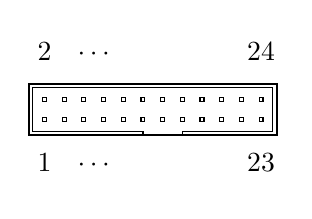
\begin{tikzpicture}[scale=.25]
		\foreach \x in {1, 2, 3, 4, 5, 6, 7, 8, 9, 10, 11, 12} {
			\foreach \y in {1, 2} {
				\draw (\x-.1,\y-.1) -- (\x-.1,\y+.1) -- (\x+.1,\y+.1) -- (\x+.1,\y-.1) -- cycle;
			}
		}
		%\draw         (.4,.4) -- (.4,2.6) -- (13.6,2.6) -- (13.6,.4) -- (.4,.4);
		\draw         (.4,.4) -- (.4,2.6) -- (12.6,2.6) -- (12.6,.4) -- (8,.4) -- (8,.2) -- (6,.2) -- (6,.4) -- cycle;
		\draw [thick] (.2,.2) -- (.2,2.8) -- (12.8,2.8) -- (12.8,.2) -- cycle;
		\node [below] at (1,0) {\strut1};
		\node [above] at (1,3) {\strut2};
%		\node [below] at (2,0) {\strut3};
%		\node [above] at (2,3) {\strut4};
		\node [below] at (3.5,0) {\strut$\cdots$};
		\node [above] at (3.5,3) {\strut$\cdots$};
		\node [below] at (12,0) {\strut 23};
		\node [above] at (12,3) {\strut 24};
	\end{tikzpicture}
\end{center}
For readerboards before version 2.1.0, this 24-position ribbon cable carries signals to directly drive the 64$\times$8 \acronym{LED}
matrix.  The other end of this cable mates with J0 on the shield board. The pinout of its \acronym{IDC} header  is:
\begin{center}
	\begin{tabular}{rl|rl|rl|rl}
		1&D6     & 7&RCLK                          &13&+5\,V DC&19&Gnd\\
		2&D5     & 8&D2                            &14&+5\,V DC&20&Gnd\\
		3&D7     & 9&$\overline{\hbox{\mc{G}}}$    &15&+5\,V DC&21&R2\\
		4&D4     &10&D1                            &16&+5\,V DC&22&REN\\
		5&SRCLK  &11&$\overline{\hbox{\mc{SRCLR}}}$&17&Gnd     &23&R1\\
		6&D3     &12&D0                            &18&Gnd     &24&R0\\
	\end{tabular}
\end{center}
\subsection{Discrete LEDs (10-pin ribbon cable) [1.0.1 J2, 2.0.0 J2]}
%
%   . . . . . . . . . . . . .
%   . . . . . . . . . . . . .
%
\begin{center}
	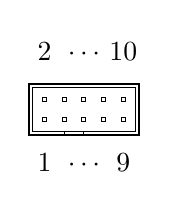
\begin{tikzpicture}[scale=.25]
		\foreach \x in {1, 2, 3, 4, 5} {
			\foreach \y in {1, 2} {
				\draw (\x-.1,\y-.1) -- (\x-.1,\y+.1) -- (\x+.1,\y+.1) -- (\x+.1,\y-.1) -- cycle;
			}
		}
		%\draw         (.4,.4) -- (.4,2.6) -- (13.6,2.6) -- (13.6,.4) -- (.4,.4);
		\draw         (.4,.4) -- (.4,2.6) -- (5.6,2.6) -- (5.6,.4) -- (2,.4) -- (2,.2) -- (3,.2) -- (3,.4) -- cycle;
		\draw [thick] (.2,.2) -- (.2,2.8) -- (5.8,2.8) -- (5.8,.2) -- cycle;
		\node [below] at (1,0) {\strut1};
		\node [above] at (1,3) {\strut2};
%		\node [below] at (2,0) {\strut3};
%		\node [above] at (2,3) {\strut4};
		\node [below] at (3,0) {\strut$\cdots$};
		\node [above] at (3,3) {\strut$\cdots$};
		\node [below] at (5,0) {\strut 9};
		\node [above] at (5,3) {\strut 10};
	\end{tikzpicture}
\end{center}
For readerboards before version 2.1.0, this 24-position ribbon cable carries signals to directly drive the 64$\times$8 \acronym{LED}
matrix.  The other end of the cable mates with J1 on the shield board. The pinout of its \acronym{IDC} header  is:
\begin{center}
	\begin{tabular}{rl|rl}
		1&GND& 6&L6\\
		2&GND& 7&L2\\
		3&L0 & 8&L5\\
		4&L7 & 9&L3\\
		5&L1 &10&L4\\
	\end{tabular}
\end{center}
\subsection{Board Power (3-pin screw terminal) [1.0.1 J0, 2.0.0 J0]}
This 3-position screw terminal block provides power to the readerboard. Note that the +5\,V supply is also connected
to pins 13--16, and Ground to pins 17--20 of J1, the only power required here is the +9\,V input that drives the \acronym{LED}s themselves.
\begin{center}
	\begin{tabular}{rl}
		1&+5\,V DC in\\
		2&GND\\
		3&+9\,V DC in\\
	\end{tabular}
\end{center}

\subsection{Shield Power (5-pin screw terminal) [Shield J2]}
This 5-position screw terminal block accepts incoming +9\,V DC power and ground on pins 4 and 3 respectively. It then provides
+5\,V DC, +9\,V DC, and ground outputs on pins 1, 2, and 5 respectively to supply power to the main display board.
\begin{center}
	\begin{tabular}{rl}
		1&+5\,V DC out\\
		2&GND\\
		3&GND\\
		4&+9\,V DC in\\
		5&+9\,V DC out\\
	\end{tabular}
\end{center}

\subsection{Shield RS-485 (6-pin screw terminal) [Shield J4]}
This 6-position screw terminal block accepts incoming RS-485 signals A, B, and ground on pins 2, 1, and 3 respectively, and outputs
the network signals A, B, and ground on pins 6, 5, and 4 respectively, to go on to the next device in the chain. If this is the last
device, then nothing should be connected to pins 5 and 6. Instead, install jumper J5 which connects a 120$\Omega$ resistor across
those terminals to terminate the network at that point.
\begin{center}
	\begin{tabular}{rl}
		1&B (Data In --)\\
		2&A (Data In +)\\
		3&GND\\
		4&GND\\
		5&B (Data Out --)\\
		6&A (Data Out +)\\
	\end{tabular}
\end{center}

%\input pinouts

\indexintoc

\printindex
\end{document}
